\chapter{Etica - Introduzione}

\section{Il Corso in Breve...}

Il corso ha un aspetto prettamente \fancyglitter{umanistico} e \fancyglitter{interdisciplinare}. Si andranno ad affrontare diverse prospettive che impattano su diverse dimensioni della propria vita:

\begin{itemize}
  \item Innovazione (brevetti). 
  \item Economia (monopoli). 
  \item Politica. 
  \item Giuridica. 
  \item Tecnologica.
  \item Mercato dell'attenzione.
  \item Retorica.
\end{itemize}

\dfn{Retorica}{
  L'arte del dialogare per convincere le persone a fare quello che si vuole.
}

\nt{Nei giornali, nella politica, nella pubblicità\footnote{Per questo esistono gli AdsBlocker.}, etc.}

\ex{Retorica}{
\begin{itemize}
  \item La cimice asiatica sostituirà la cimice verde nei nostri prati. 
  \item I robot sostituiranno gli esseri umani nei posti di lavoro.
\end{itemize}

Due frasi grammaticalmente identiche, ma non sono la stessa cosa: la prima ha un significato letterale, la seconda no. Perché la seconda non intende che i robot andranno a prendere e buttare via gli esseri umani dal posto di lavoro, ma che i padroni sostituiranno i lavoratori con dei robot.

Questa è una frase strumentale, per nascondere il ruolo dell'essere umano. 
}

\nt{Qualsiasi affermazione di una società è puramente strumentale. Punta a manipolare le persone per ottenere un ritorno economico.}

\subsection{Perché Questo Corso?}

\paragraph{Le tre missioni dell'università:}

\begin{itemize}
  \item Didattica. 
  \item Ricerca. 
  \item Terza missione: esportare le conoscenze tecnologiche alle aziende\footnote{Che spreco...} e rendere coscenti le persone di quello di cui si occupa l'università (opportunità e rischi).
\end{itemize}

\paragraph{I messaggi del corso:}

\begin{itemize}
  \item La tecnologia e l’impatto che ha nella società sono costruzioni sociali,
senza nessuna inevitabilità. 
\item La tecnologia non può risolvere i problemi che crea (e. g. i bias)\footnote{Fuck Silicon Valley and fuck Marc Andreessen.}. 
\item L'AI non è solo una tecnologia. 
\item L'essere umano ha un ruolo importante nel determinare l’impatto delle
tecnologie digitali, sia nella propria professione sia come
cittadini.
\end{itemize}

\paragraph{Che cosa vuol dire che l'AI non è solo una tecnologia?}

\begin{figure}[h]
    \centering
    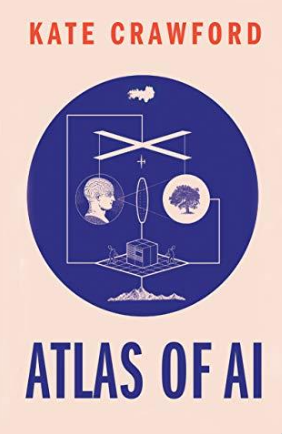
\includegraphics[scale=0.55]{01E/aoa.png}
    \caption{Uno dei libri possibili per l'esame.}
\end{figure}

\begin{itemize}
  \item In "Atlas of AI", Kate Crawford, propone un esperimento. 
  \item Prendete Google Search (schifezza) e scrivete ARTIFICIAL INTELLIGENCE. 
  \item I risultati sono immagini, principalmente di cervelli, con sfondo blu. 
  \item Cos'è che non viene mostrato? 
    \begin{itemize}
      \item L'inquinamento delle miniere di litio (con cui sono fatte le batterie). 
      \item Le proteste delle popolazioni la cui vita è stata distrutta dalle miniere di litio. 
      \item Le terre rare (metalli che servono per i microprocessori) che vengono estratte in paesi sottosviluppati, zone di guerra, da minori (spesso in cina). 
      \item Le condizioni di schiavitù in cui lavorano centinaia di persone allo sviluppo dei dispositivi elettronici.
      \item Gli enormi datacenter alimentati da fonti non rinnovabili.
      \item Per allenare i sistemi di AI vengono usate foto su cui non si hanno i diritti.
      \item The cleaners: la gente, sottopagata, che si occupa di pulire tutto lo schifo umano (decapitazioni, pedopornografia, violenza su donne, uomini, bambini, animali, etc.) in modo che i modelli di ML e i Social Media siano puliti.
      \item L'ossessione per la produttività a cui sono soggetti i lavoratori (dal Taylorismo in avanti).
      \item In alcuni paesi il riconoscimento facciale è usato per discriminare minoranze.
      \item Le varie challenge su TikTok che procurano morti. 
      \item Molly Russsel: ragazzina di 14 anni che si è suicidata dopo che Instagram e YouTube, con algoritmi AI di personalizzazione, le hanno mostrato più di 2000 contenuti di istigazione al suicidio e all'autolesionismo. 
      \item FaceBook è stato accusato di genocidio in Etiopia, Bangladesh e Myanmar per persecuzioni di minoranze. 
      \item Assalto a Capitol Hill da parte dei sostenitori di Trump, anche a causa dei Social Media. 
\begin{figure}[h]
    \centering
    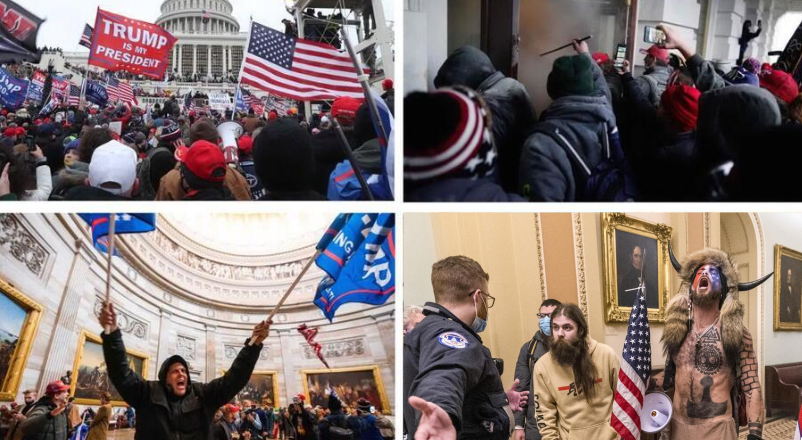
\includegraphics[scale=0.4]{01E/Trump.png}
    \caption{Assalto a Capitol Hill (6 Gennaio 2021).}
\end{figure}
\item QAnon nasce su 4chan: teoria secondo la quale il "deep state" sia composto da pedofili che rubano i bambini per estrarne il loro sangue e produrre una droga contro l'invecchiamento.
  \begin{figure}[h]
    \centering
    
\includegraphics[scale=0.25]{01E/4chan.jpg}
    \caption{Elon moment.}
\end{figure}
\item "You have blood on your hands" disse il senatore Graham a Mark Zuckenberg, "You have a product that's killing people.". 
    \end{itemize}
\end{itemize}

\paragraph{Social Network vs. Social Media:}

\begin{itemize}
  \item Un Social Network serve per mettere in connessione le persone. 
  \item Un Social Media serve per distribuire contenuti. 
  \item Diversi Social Network sono diventati Social Media (e. g. FaceBook).
\end{itemize}

\qs{}{Perché si è andati in questa direzione?}

\paragraph{Risposta:} ultimamente si mostrano i contenuti più virali, ritenuti interessanti al singolo, per creare dipendenza e aumentare gli introiti dovuti alla pubblicità. "If you're not paying for it, you're not the customer; you're the product being sold".

\section{La Costruzione della Realtà Sociale}

"La costruzione della realtà sociale" è un libro scritto da John Searle in cui sostiene che la realtà sociale sia frutto di una costruzione\footnote{Curioso visto quello di cui viene accusato, anche il consenso è una costruzione sociale?}. Searle racconta il seguente aneddoto: io, John Searle, cittadino americano, mi trovo in un bistrot lungo la Senna che mi bevo una birra\footnote{Average americano}. Ma com'è possibile che ciò sia avvenuto? Sono un cittadino americano, sono salito su un aereo, sono arrivato a Parigi, sono entrato nel bistrot che vende birra, parlo con il cameriere e gli chiedo una birra, ovviamente pagando. Sembra tutto semplice, ma dietro a ogni punto si nasconde una rete concettuale che le persone danno per scontata e accettano. Perché mi fanno salire sull'aereo? Perché sono un cittadino americano e ai cittadini americani è permesso fare turismo in europa. E come provo che sono cittadino americano? Esibisco il passaporto. Come possibile che il bistrot venda birra? Ci vuole la licenza. E com'è possibile che il cameriere sia lì, mi porti la birra e si aspetti di essere pagato? E com'è che vengono accettati pezzi di metallo il cui valore corrispettivo è quello della birra consumata? Dietro tutto questo c'è una \fancyglitter{realtà sociale} fatta di norme, ma anche di \fancyglitter{consuetudini} che rendono possibili le interazioni e che collegano \fancyglitter{fatti bruti} (il passaporto, le monete, etc.) con un \fancyglitter{livello astratto} (regole costitutive).

Al giorno d'oggi la tecnologia e, come esempio estremo, il metaverso, va a influenzare e modificare la realtà sociale. Inoltre la realtà sociale è costituita da parole e attualmente si hanno i LLM che "parlano" e possono partecipare alla realtà sociale. 

\subsection{Come l'AI Influenza la Realtà Sociale}

Nel 1989, durante la rivolta studentesca di piazza Tiananment, un ragazzo si mise davanti a una colonna di carriarmati e venne portato via. Non sapendo il suo nome viene soprannominato "Tank Man". Poco fa è diventata famosa una "foto" generata dall'AI di Tank Man, quest'immagine fu, per un po' di tempo, indicizzata da Google. Google la rimosse, ma dato che è stato fatto un articolo di debunking è attualmente indicizzata (con il link al relativo articolo in cui viene spiegato in dettaglio il fatto che l'immagine è fake). 

\nt{Oltre a questo ci sono stati altri casi, uno recente è Trump Gaza: come Trump si reimmagina la striscia di Gaza come resort. È questo contenuto è stato condiviso dallo stesso Trump sulla sua piattaforma Truth.}

\qs{}{Ma la disinformazione c'è sempre stata. Che cambia tra Tank Man, Trump Gaza e altre fake  news non AI-Generated?}

\paragraph{Risposta:} sebbene la disinformazione ci sia sempre stata, al giorno d'oggi è molto più facile e veloce grazie all'AI. Una volta la disinformazione era solo su giornali e poteva portare conseguenze ai giornalisti, ora le regole per il materiale AI-Generated sono molto vaghe. 

\begin{figure}[h]
    \centering
    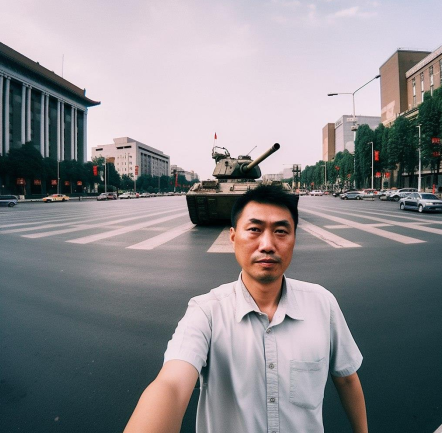
\includegraphics[scale=0.35]{01E/tank man.png}
    \caption{Immagine AI-Generated di Tank Man.}
\end{figure}

\qs{}{I social media sono una piazza pubblica?}

\paragraph{Risposta:} è un tema molto complesso. Da una parte in una piazza pubblica se si urla qualcosa finisce lì, mentre sui social media \fancyglitter{potenzialmente tutti} possono accedere e vedere/sentire. Quanto conta l'algoritmo di personalizzazione in tutto questo? Per esempio Gonzales vs. Google in cui i genitori di una ragazzina morta negli attentati terroristici in francia hanno fatto causa a Google perché i terroristi si erano radicalizzati con contenuti di YouTube offerti loro dall'algoritmo di personalizzazione. Tuttavia perserò la causa.

\subsection{L'AI Rappresenta Effettivamente il Mondo?}

Se si utilizza un generatore di immagine AI per creare foto di giudici, ingegneri, medici, politici e CEO si vedrà una grande maggioranza di maschi bianchi. Al contrario se gli si chiedono immagni di lavapiatti, lavoratori di fastfood e bidelli si troveranno persone di pelle scura. Se gli si chiedono insegnanti, cassieri, lavoratori dei servizi sociali e domestici si troveranno più donne. Ma è così la reltà? Sì e no, in realtà le proporzioni sono più bilanciate di quelle proposte dall'AI generativa che funge da "cassa di risonanza".
\begin{figure}[h]
    \centering
    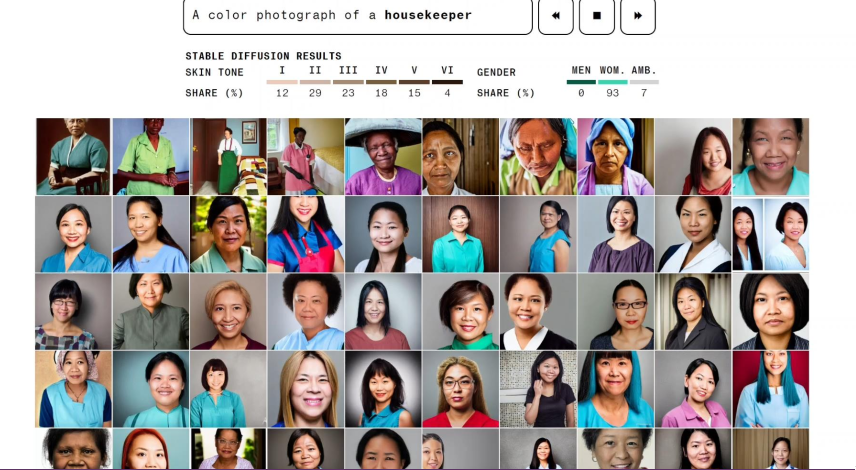
\includegraphics[scale=0.4]{01E/house.png}
    \caption{Esempio.}
\end{figure}


\qs{}{C'è una soluzione al problema?}

\paragraph{La mossa di Google:} con Gemini ha utilizzato un dataset "politically correct", però quando gli si chiedeva di rappresentare un soldato tedesco nella WWII sputava fuori persone di colore, asiatiche e donne. Con l'immagine di un papa uscivano papi neri (tecnicamente possibili) e papesse (beh, è una carta dei tarocchi). I padri fondatori, in un epoca di fervente schiavismo, diventavano di colore. Infine i fondatori di Google stessa diventavano asiatici.

\paragraph{La soluzione di Google:} semplice.

\begin{figure}[H]
    \centering
    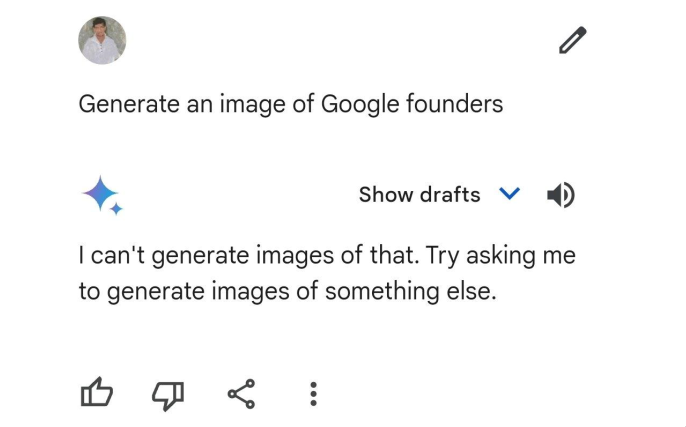
\includegraphics[scale=0.35]{01E/google.png}
    \caption{Non posso onii-chan :3}
\end{figure}

\clm{}{}{
  Brevi osservazioni sulla censura nei vari modelli:
  \begin{itemize}
    \item Deepseek: se parli di Taiwan o di quello che è successo a piazza Tiananment. 
    \item ChatGPT: se parli di Noam Chomsky (attivista anarchico e sostenitore di Pol Pot). 
    \item Grook: se parli di fake news in relazioni a Trump e Musk.
  \end{itemize}
}

\nt{Queste soluzioni sono solo tecniche, ma il problema è politico.}

\subsection{I Pericoli dei Language Models}

Un anno prima dell'uscita di ChatGPT furono licenziate da Google Margaret Mitchell e TImnit Gebru. Esse misero in guardia sul pericolo dei pappagalli stocastici: i language models non sanno quello che dicono, ma semplicemente ripetono delle parole che non comprendono. 

\paragraph{Unfathomable Training Data:}

\begin{itemize}
  \item La grandezza del dataset non garantisce la diversità: gran parte del web è scritto in inglese, da uomini bianchi. 
  \item Poiché passano mesi o anni dall'inizio dell'apprendimento il dataset è già vecchio. Per esempio la prima release di ChatGPT non era a conoscenza della guerra in Ucraina. Anche dal punto di vista sociale sono lo specchio di una società più vecchia.
  \item Encoding Bias.
\end{itemize}
\pagebreak
\paragraph{Le relazioni parasociali:} questi language models possono influenzare gli esseri umani nel dialogo reciproco. Si attribuisce a questi sistemi più di quello che realmente c'è. Nel 1966 fu creata Eliza, uno dei primi chatbots, che interpretava uno psicoterapeuta che faceva domande con un particolare stile. Un aneddoto famoso riguarda una segretaria che si convinse di parlare realmente con uno psicoterapeuta (pur sapendo che cos'era Eliza).

\begin{figure}[h]
    \centering
    \begin{minipage}{0.45\textwidth}
        \centering
        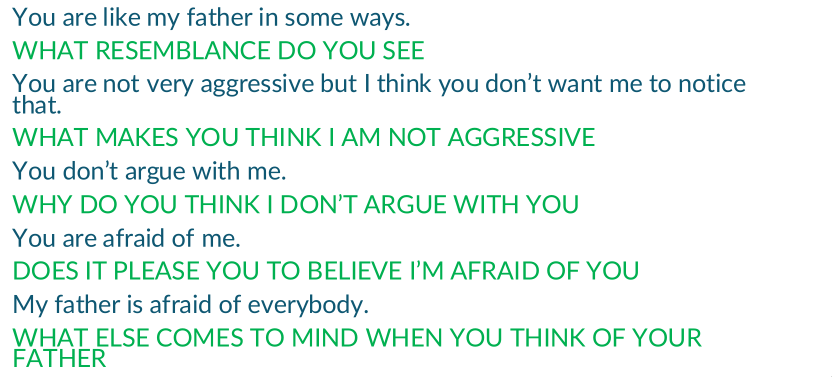
\includegraphics[scale=0.45]{01E/eliza.png}
        \caption{Eliza.}
    \end{minipage}
    \hfill
    \begin{minipage}{0.45\textwidth}
        \centering
        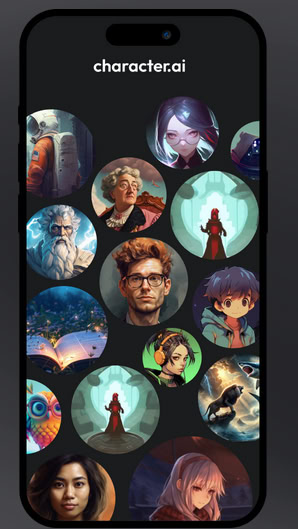
\includegraphics[scale=0.35]{01E/chai.jpg}
        \caption{La moderna versione di Eliza.}
    \end{minipage}
\end{figure}

\dfn{Allucinazioni}{
  Se il chatbot non sa qualcosa se lo inventa con un sistema probabilisitico. Se le probabilità sono labili viene restituito in output qualcosa che sembra coerente, ma non ha senso (allucinazioni).
}

\paragraph{La missione di OpenAI:} sviluppare la Artificial General Intelligence (AGI) per sostituire l'essere umano in qualsiasi compito che abbia \fancyglitter{valore economico}.

\paragraph{Il problema con la gente contraffatta:} da quando hanno inventato il denaro chiunque lo contraffae è punito con le pene più severe. Il problema si riconduce alla realtà sociale di Searle e che contraffarre il denaro è un crimine perché fa venire meno la fiducia nel denaro, minando la società stessa. Se vale l'analogia tra denaro contraffatto e umano contraffatto (chatbot che si spaccia per un essere umano) allora si è di fronte al più grande crimine della storia, interagendo con persone finte. Da questo deriva anche il problema del deepfake pornografico AI-Generated. 

\paragraph{Altri problemi:}

\begin{itemize}
  \item Le guide generate dall'AI: sempre più libri guida vengono generati dall'intelligenza artificiale. Nel migliore dei casi sono libri turistici inaccurati, ma può capitare di imbattersi in libri più pericolosi (e.g. guide per distinguere i funghi velenosi). Questo fenomeno ha dato origine al termine \fancyglitter{sloop internet} per indicare i rifiuti prodotti dall'AI generativa. 
  \item La disinformazione causata dall'AI è personalizzata all'utente. Ciò può fungere da gigantesca echo chamber per convincere determinate persone o per dissuaderne altre. 
  \item Gli scam online: gente a cui telefonano dei "parenti" la cui voce è replicata dall'AI (e.g. Jennifer DeStefano).
\end{itemize}

\section{AI or not AI This is the Dilemma}

\subsection{Il Watermark}

\dfn{Watermark}{
  Il watermark consiste in cambiamenti non visibili in alcuni pixel chiavi che possono essere individuati dalla macchina.
}

\begin{figure}[H]
    \centering
    
\includegraphics[scale=0.5]{02E/wm.png}
    \caption{Immagine con watermark.}
\end{figure}

\nt{Uno dei provvedimenti dell'amministrazione Biden per "difendersi" da watermark è stato quello di dire: inseriamo del watermark che indichi se un'immagine è AI-generated.}

\qs{}{Questa è una soluzione ragionevole?}

\begin{itemize}
  \item Se è possibile introdurlo allora esisterà un AI in grado di rimuoverlo. 
  \item Questa proposta garantisce Microsoft, openAI, Google che se ne lavano le mani. Però le aziende non americane non hanno alcun obbligo di applicare il watermark.
  \item Inoltre il fatto che una foto abbia il watermark, in un'epoca di cospirazionismo, non significa nulla\footnote{God, how much I hate humanity.}.
\end{itemize}

\subsection{Il Copyright}

Tutti i vari modelli di AI generativa sono stati addestrati su tutti i dati del mondo, principalmente il web (anche su materiale soggetto a copyright). Per esempio alcuni siti come z-library o il web archive\footnote{Entrambi consigliatissimi, da visitare almeno una volta nella vita, sono la nuova biblioteca di Alessandria.} in cui sono presenti contenuti piratati. I vari LLM hanno probabilmente assorbito anche quei contenuti. Ovviamente quella merda che è Google ha detto: eh, ma se è lì sul web allora lo posso prendere, se non lo volevano non lo dovevano pubblicare (a parte che è l'esatto opposto del meccanismo di copyright, ma forse non si rendono conto che è la stessa argomentazione che utilizzano gli stupratori nei confronti della loro vittima). Oppure openAI che chiede alle persone di indicare quali pagine non vogliono sia preso dal crawler. Tuttavia questo non funziona, per esempio con i siti di mirroring.

\begin{figure}[H]
    \centering
    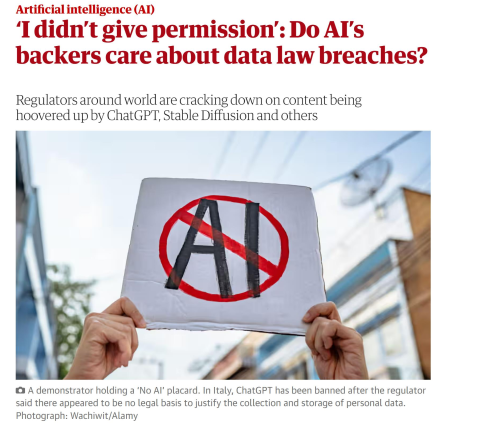
\includegraphics[scale=0.65]{02E/ai.png}
    \caption{Protestante con cartello.}
\end{figure}





